\par Evidence for the charged Higgs boson was searched for in events in which the Higgs boson 
decays to a $\tau$ lepton and a $\nu_\tau$. In these events, the $\tau$ lepton decays hadronically 
and is reconstructed as a $\tauvis$. The 4FS and 5FS topologies for such events, signal events, are 
respectively  

\begin{equation}
gb\to[t][H^+]\to[(jj)b][(\tauvis+\met)]
\label{eq:topA}
\end{equation} 
and 
\begin{equation}
gg\to[tb][H^+]\to[(jj)bb][(\tauvis+\met)].
\label{eq:topB}
\end{equation}

In the terminology of Equations~\ref{eq:topA} and~\ref{eq:topB} a $b$-tagged reconstructed jet 
is represented by $b$, otherwise it is represented by $j$. 
Table~\ref{tab:sigReg} summarizes the selection criteria optimized to select signal events as represented by 
 Equations~\ref{eq:topA} and~\ref{eq:topB} and minimize the level of background contamination. These 
selection criteria define the {\it signal region}. This section 
discusses each component of these selection criteria.  

\par Before pre-selection, measures were taken to reduce the number of events originating 
from instrumental effects such as intra-beam interactions and proton losses upstream of the 
interaction point.\footnote{Proton losses from the beam may induce cascades that may 
eventually reach the ATLAS detector. These cascades would be reconstructed as jets.} 
 This was achieved by requiring the following :

\begin{enumerate}
\item no jet with $\pT>25~\GeV$ that fails 
the \texttt{BadLoose} quality selection criteria discussed in Section~\ref{sec:jets}; 
\item at least one vertex with two or more tracks. This selection is designed to identify the primary 
vertex to which all the physics objects should point; 
\item the SCT, Tile and LAr Calorimeters not be in an error or unknown state; 
\item and the event must be considered {\it complete} by the TTC.\footnote{See Section~\ref{sec:trigger} 
for a more formal definition of `complete'.}
\end{enumerate}

These selection criteria are collectively referred to as {\it clean-event} in the rest of 
this chapter. 

\begin{table}[!h]
\centering
  \resizebox{\textwidth}{!}{
   \begin{tabular}{|l|r|}
\hline
            								& Selection \\
\hline\hline
\multirow{4}{*}{pre-selection}& Pass trigger \texttt{HLT\_xe70\_tc\_lcw}(\texttt{HLT\_xe90\_mht}) for 2015(2016) data \\
															& Exactly one $\tauvis$ with $\pt>40$~\GeV \\ 
															& At least 3 jets with $\pt>25$~\GeV \\
															& No muon or electron \\ 
\hline
\multirow{3}{*}{full selection} & At least one $b-$tagged jet \\				
																& $\met>150$ GeV \\
																& $\mT>50$ GeV \\
\hline 
   \end{tabular}
}
\caption{Signal region definition. Additionally, measures were taken to ensure that events originated 
from inelastic $pp$ collisions and no jets originated from unwanted experimental effects.}
\label{tab:sigReg}
\end{table}

\par The event topology presented in Equations~\ref{eq:topA} and~\ref{eq:topB} suggests several options 
to trigger on when selecting such events. One could use a trigger that demands presence of a $\tauvis$, some \met, 
or both the $\tauvis$ and some $\met$. The least stringent $\tauvis$-only trigger available on both the 
2015 and 2016 trigger menu required presence of a $\tauvis$ with $\pT>160~\GeV$ in the event. Since the topology 
in Equations~\ref{eq:topA} and~\ref{eq:topB} is not biased towards high-\pt\ $\tau$ leptons, a $\tauvis$-only 
trigger was not chosen. The least stringent of all unprescaled triggers that require presence of both a $\tauvis$ 
and some $\met$ required the $\tauvis$ to have at least 35~\GeV\ in \pt\ and $\met>70~\GeV$. Likewise, the least stringent 
unprescaled trigger that requires the presence of just \met\ required $\met>70~\GeV$. The efficiencies of the \met-only and 
the \met+\tauvis\ triggers when selecting signal events in Monte Carlo simulation were found to be comparable. Thus, there was 
no advantage in using an \met+\tauvis\ trigger over an \met-only trigger. 

\par To avoid imposing selection criteria on the \tauvis, only \met-only-based triggers were considered.  
Figure~\ref{fig:trigComp} shows signal selection efficiency distributions for several of \met-only triggers 
on a signal sample with $\mcH=200$~\GeV, binned in \met. The naming convention for these triggers can be  
generalized to
\begin{center}
 \texttt{Level\_xeMissingEnergyCut\_MissingEnergyReco}.
\end{center}
\texttt{Level} indicates the level in the trigger 
system at which the trigger is active. In this case, the level is \texttt{HLT}, denoting the Higher Level Trigger. At 
this level the \met\ may be reconstructed using either topological clusters, in which case 
\texttt{MissingEnergyReco} is \texttt{tc\_lcw}, or jet energies, in which case  
\texttt{MissingEnergyReco} is \texttt{mht}. Otherwise, the \met\ is reconstructed using energy recorded in 
calorimeter cells. For $100<\met<200$~\GeV, 
the most efficient trigger is \texttt{HLT\_xe70\_tc\_lcw}, which accepts events with $\met>70$~\GeV. 

\begin{figure}[!h]
\centering
   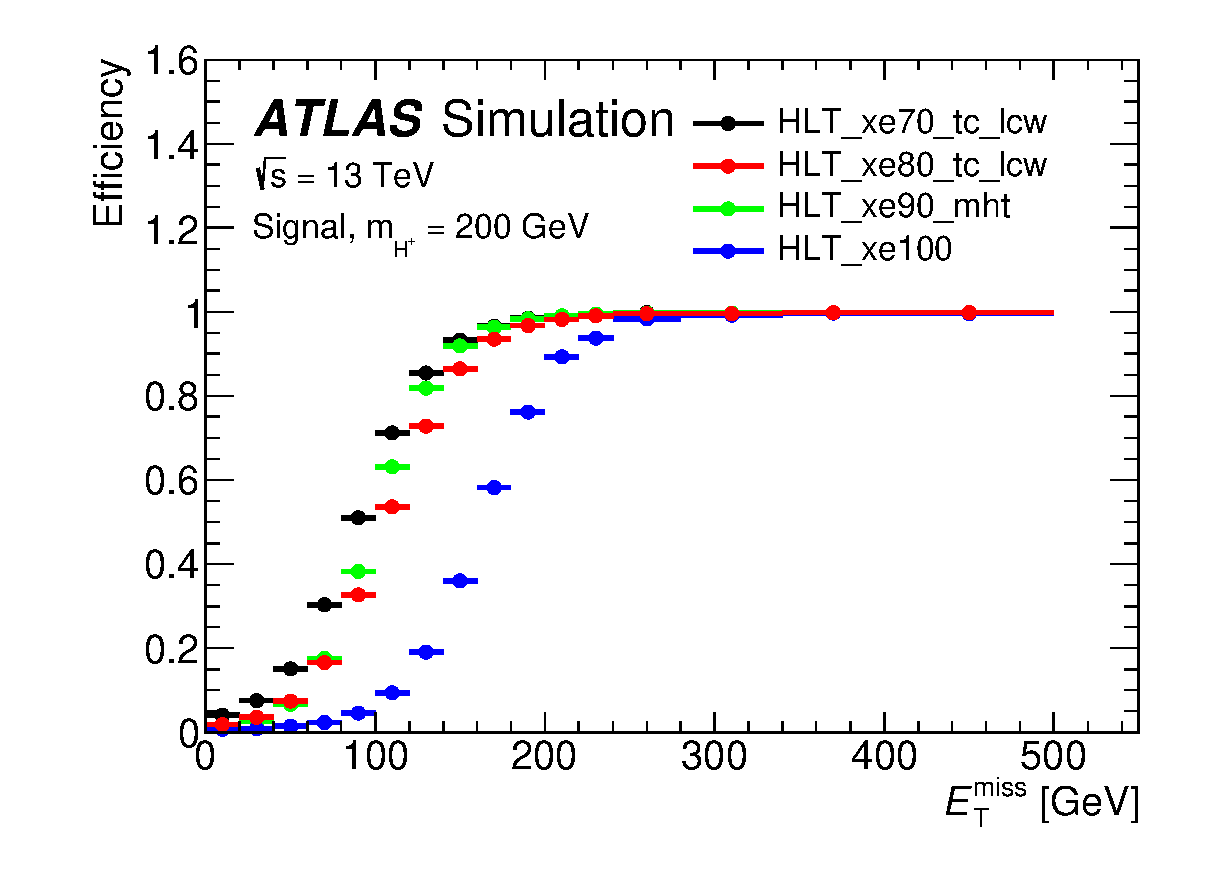
\includegraphics[width=0.8\textwidth]{figures/mh200_xe70_xe90_xe100_xe80.eps}
\caption{Plots of the efficiencies of several \met-based triggers, obtained from simulation of signal with $\mcH=200~\GeV$}
\label{fig:trigComp}
\end{figure}
 
\par While \texttt{HLT\_xe70\_tc\_lcw} was the least stringent \met-only trigger during the 2015 data-taking period, 
\texttt{HLT\_xe90\_mht} was the least stringent in the 2016 data-taking period. 
Events from the 2015 data-set were therefore triggered with \texttt{HLT\_xe70\_tc\_lcw}, and events from the 
2016 data-set were triggered with \texttt{HLT\_xe90\_mht}.
 
\par In addition to trigger requirements, the pre-selection criteria required  
events to have exactly one $\tauvis$. The said \tauvis\ was also required to have $\pt>40$~\GeV. 
At least 3 reconstructed jets with $\pt>25$~\GeV\ were required to be present. 
Since the topologies in Equations~\ref{eq:topA} and ~\ref{eq:topB} do 
not include electrons or muons, the event was also required to have no electrons or muons.  

\par For the full selection at least one $b-$tagged jet was demanded. Additionally, the event had 
to have $\met>150$~\GeV\ and
 $\mT>50$~\GeV, where \mT\ is the transverse mass of the $\tauvis,\met$ system :

\begin{equation}
\mT = \sqrt{2\pt^\tau\met(1-\cos\Delta\phi_{\tau,\met})}.
\end{equation} 

Figures~\ref{fig:preselectA} and~\ref{fig:preselectB} show expected $\met$ and $\mT$ `n-1'
 distributions after the full selection criteria has been applied,\footnote{These are distributions where 
all the selection criteria has been applied except the criteria based on the variable being plotted.} 
for backgrounds where the $\tauvis$ was reconstructed from a $\tau$ lepton and for 
several signal samples. Vertical black lines show the point at which \met\ and \mT\ are cut 
on. As already been predicted, it is expected that the Top background dominates, followed by the 
\Wjets\ background.

\par Treatment of backgrounds where the \tauvis\ is reconstructed from objects other 
than $\tau$ leptons is discussed in Sections~\ref{sec:jetToTau} and \ref{sec:lepToTau}.    

\begin{figure}[!h]
\begin{subfigure}{0.5\textwidth}
   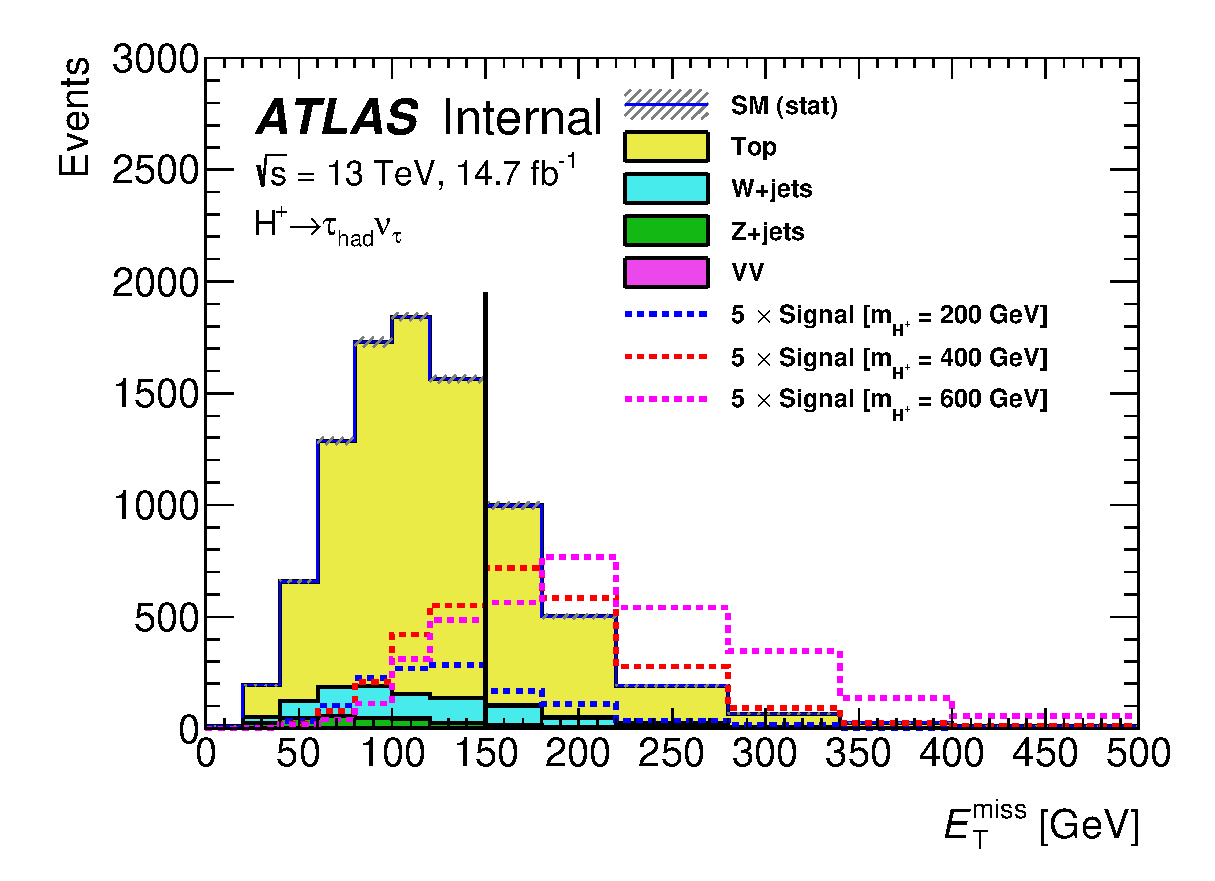
\includegraphics[width=\textwidth]{figures/met_nMinus1_expected.eps}
\caption{Expected \met\ distributions in the signal region, minus $\met>150$~\GeV}
\label{fig:preselectA}
\end{subfigure} % 
\begin{subfigure}{0.5\textwidth}
   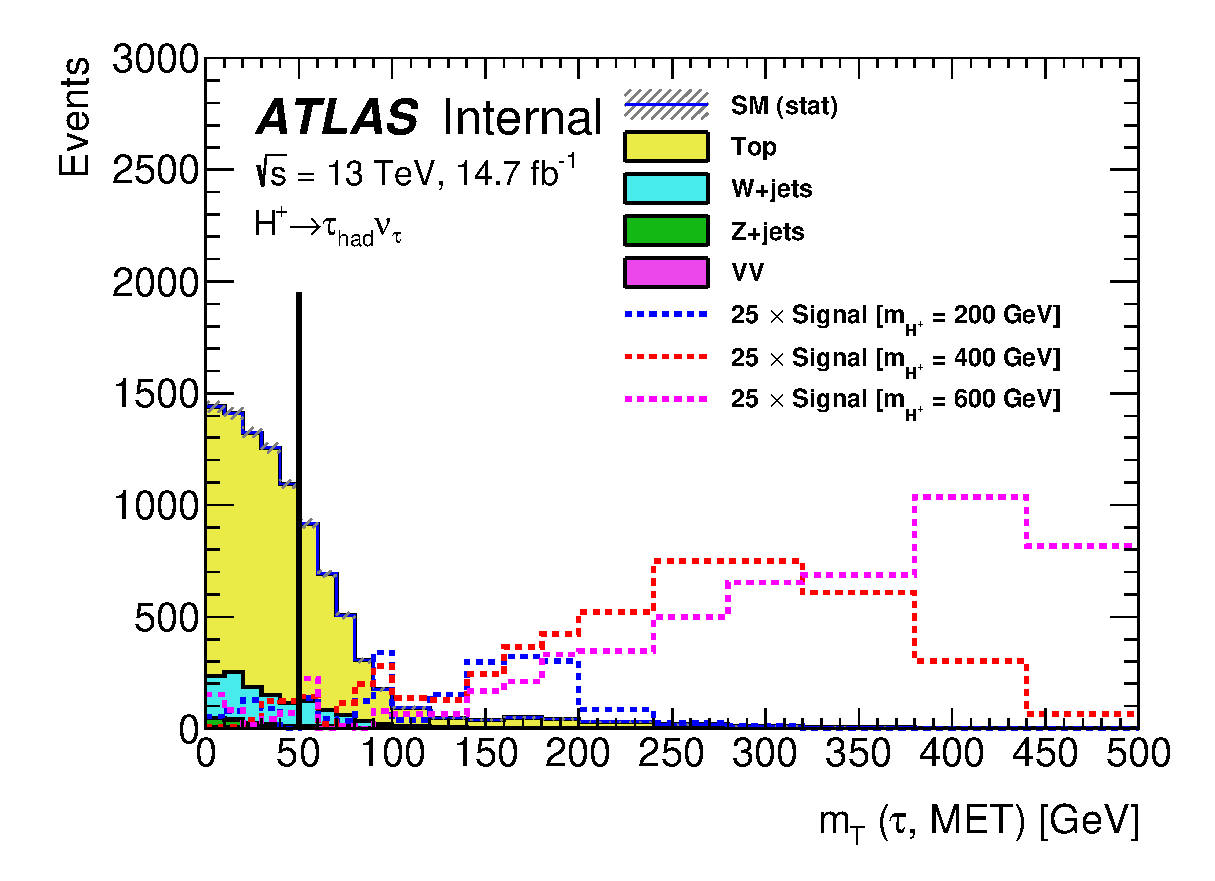
\includegraphics[width=\textwidth]{figures/mT_nMinus1_expected.eps}
\caption{Expected \mT\ distributions in the signal region, minus $\mT>50$~\GeV}
\label{fig:preselectB}
\end{subfigure}
\caption{N-1 distributions after the full selection criteria have been applied. The black 
vertical line marks the point at which the variable being plotted is cut on}
\end{figure}

Events in which \met\ is mismeasured and is aligned to the $\tau$ direction are suppressed by the \mT\ 
requirement. Moreover, events from which $\mT<50$~\GeV\ are likely to contain $\Wplus\to\tau\nu$ processes rather 
than signal. The \met\ requirement suppresses background from QCD multijets. 

%%%%%%%%%%%%%%%%%%%%%%%%%%%%%%%
%% TRIGGER EFFICIENCY STUDIES
%%%%%%%%%%%%%%%%%%%%%%%%%%%%%%%

\subsection{Trigger Efficiency}
\par Although trigger decisions in Monte Carlo simulation are sufficient to evaluate and compare trigger 
efficiencies as demonstrated by Figure~\ref{fig:trigComp}, they may not perfectly model trigger decisions 
in data. As shown in Table~\ref{tab:sigReg}, trigger decisions in simulation are essential in predicting background 
processes that contaminate the signal region. To account for this potential mis-modelling, 
efficiencies in simulation were corrected to those in data. The efficiencies from data 
were extracted from from a dedicated control region and binned in \met. The trigger 
efficiency in data, in an \met\ bin was then defined as 

\begin{equation}
\epsilon = \frac{\text{control region selection} + \text{Trigger}}{\text{control region selection}}
\end{equation}  

where the `Trigger' is either \texttt{HLT\_xe70\_tc\_lcw} or \texttt{HLT\_xe90\_mht}. Both triggers require the 
event to pass an L1 trigger that demands at least 50 GeV in online \met. Apart from passing 
the clean-event selection, the control region selection is defined as follows :
\begin{enumerate}
\item exactly one loosely identified and loosely isolated electron, trigger matched to \\ \texttt{HLT\_e26\_lhtight\_iloose\_L1EM20VH};
\item exactly one loosely identified $\tauvis$ with at least 26~\GeV;
\item and at least two reconstructed jets, one of which must be $b-$tagged.
\end{enumerate} 

\par A similar control region with exactly one muon and no electrons was also considered. 
%Without loss of generality, efficiencies from the former region are chosen. 
\mT\ and \met\ distributions in the 1-electron control region are shown in 
Figure~\ref{fig:trigReg}. Here, contributions from processes in which jets are reconstructed as \tauvis ($j\to\tau$), or 
those in which non-$\tau$ leptons are reconstructed as \tauvis ($l\to\tau$), 
were estimated using methods described in Section~\ref{sec:bkgCh}. As will become clearer in 
the said section, application of those methods in this region requires some careful extrapolations 
that compensate for differences in topological structures in the two regions. Estimations shown 
in Figure~\ref{fig:trigReg} are rather ad-hoc because they do not take into account these differences.  
Consequently, there is an obvious mis-modelling of physics processes in the low 
\met\ and \mT\ regions, as shown by the disagreement between data and simulation.
Reasonable agreement between data and predictions is observed at $\met>50$~\GeV.
Since trigger thresholds 
studied were at minimum $\met=70$, disagreements in the low \met\ and low \mT\ regions did not have significant impact on 
measurements.

\begin{figure}[!h]
\begin{subfigure}{0.5\textwidth}
   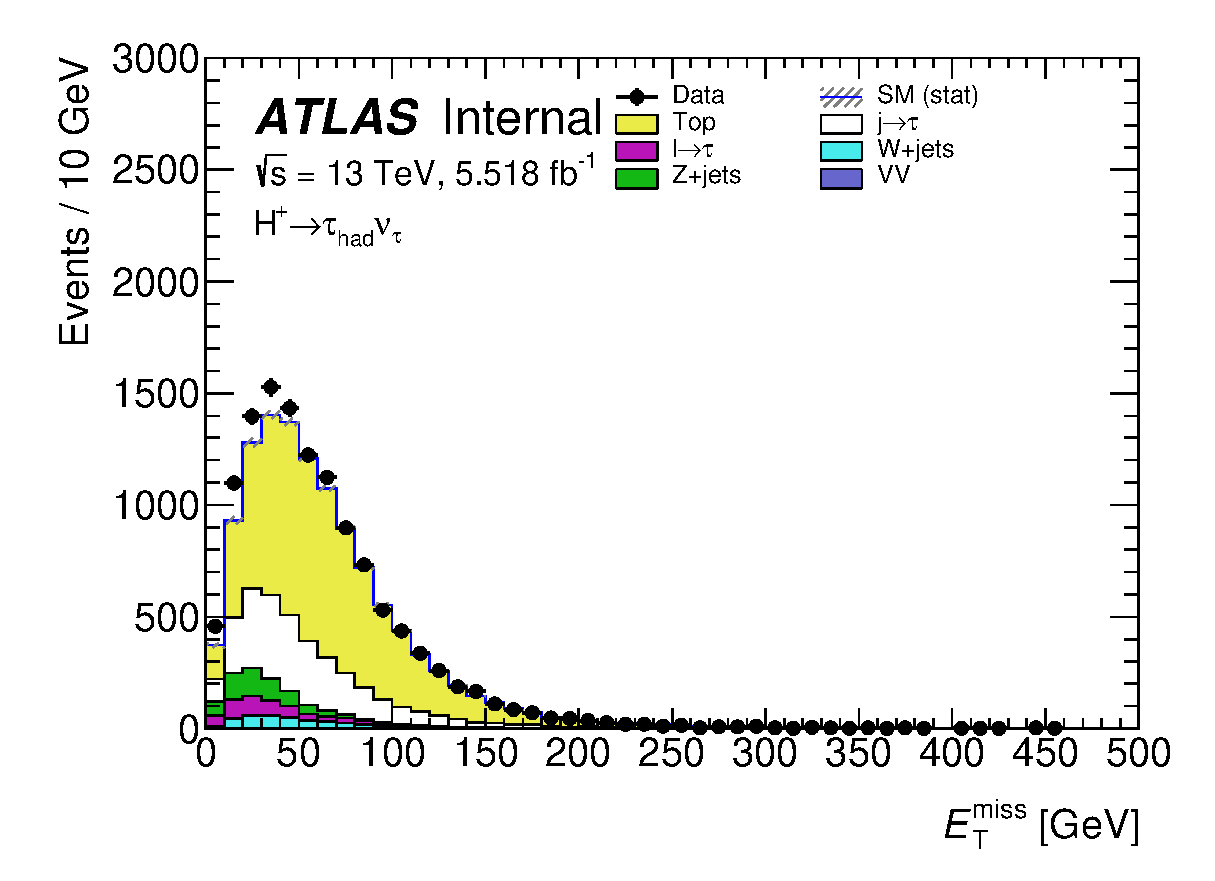
\includegraphics[width=\textwidth]{figures/all_CutNoMatchNbjets_met_lin_forTriggers.eps}
\end{subfigure} % 
\begin{subfigure}{0.5\textwidth}
   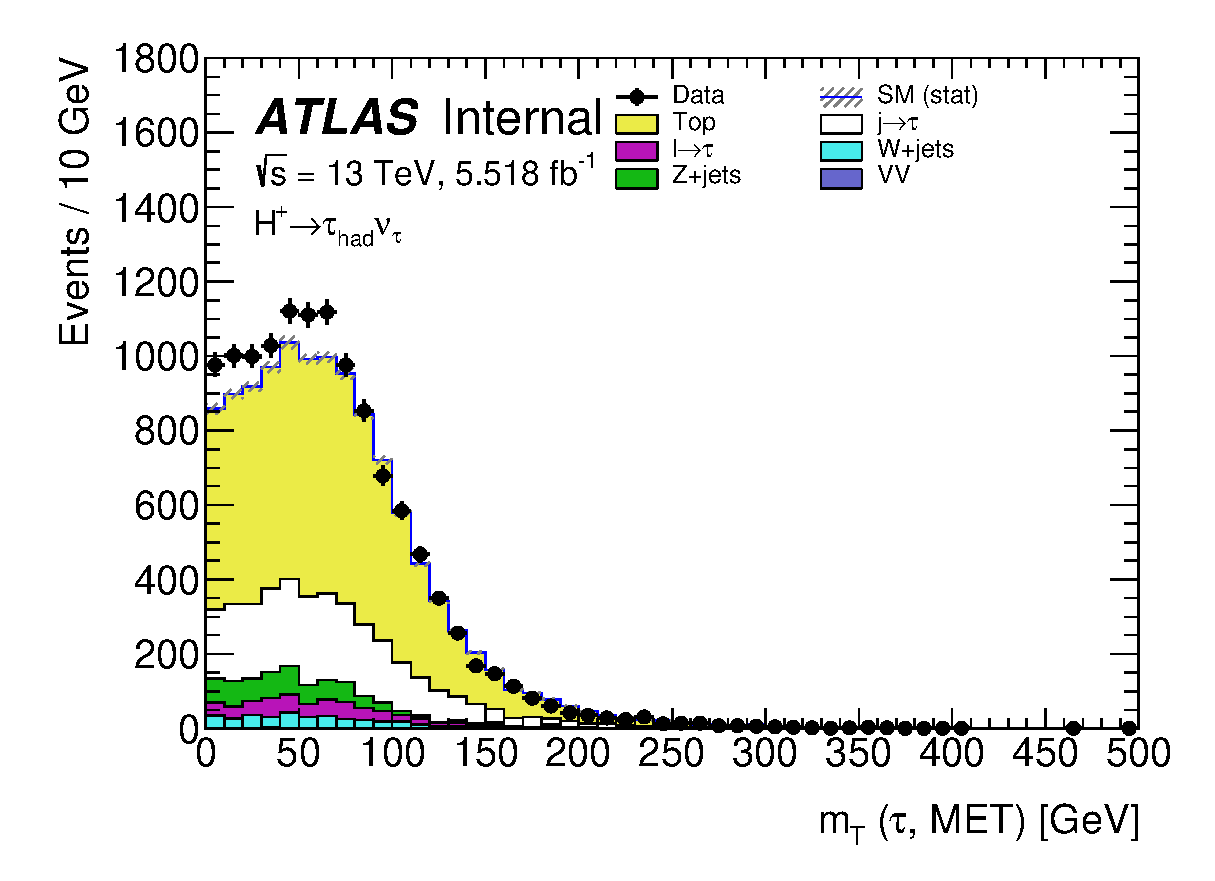
\includegraphics[width=\textwidth]{figures/all_CutNoMatchNbjets_mT_lin_forTriggers.eps}
\end{subfigure}
\caption{\met\ and \mT\ distributions in the control region used to measure trigger efficiencies. Since trigger thresholds 
studied were at minimum $\met=70$, disagreements in the low \met\ and low \mT\ regions did not have significant impact on 
measurements}
\label{fig:trigReg}
\end{figure}

\par To obtain continuous efficiency distributions, the binned efficiencies from data were
 fitted to the error function, parametrized as 

\begin{equation}
F(x) = p_0.\left [ 1 + \text{erf}\left ( \frac{x-p_1}{p_2}\right )\right ] + p_3
\end{equation}

where initial values for the $p_i$ were repeatedly changed until an optimal 
fit was obtained. The optimization of the fit was quantified by the $\chi^2$ distribution. 
This procedure was done separately for the 2015 and 2016 datasets. The efficiency 
distributions and their respective fits are shown in Figures~\ref{fig:trigFitA} and~\ref{fig:trigFitB}, 
reaching 100\% efficiency at about \met$=$250~\GeV. In these plots the region from which most of the 
events in the signal region lie, $150<\met<250~\GeV$, is marked with vertical dashed lines.  
 
\begin{figure}[!h]
\begin{subfigure}{0.5\textwidth}
   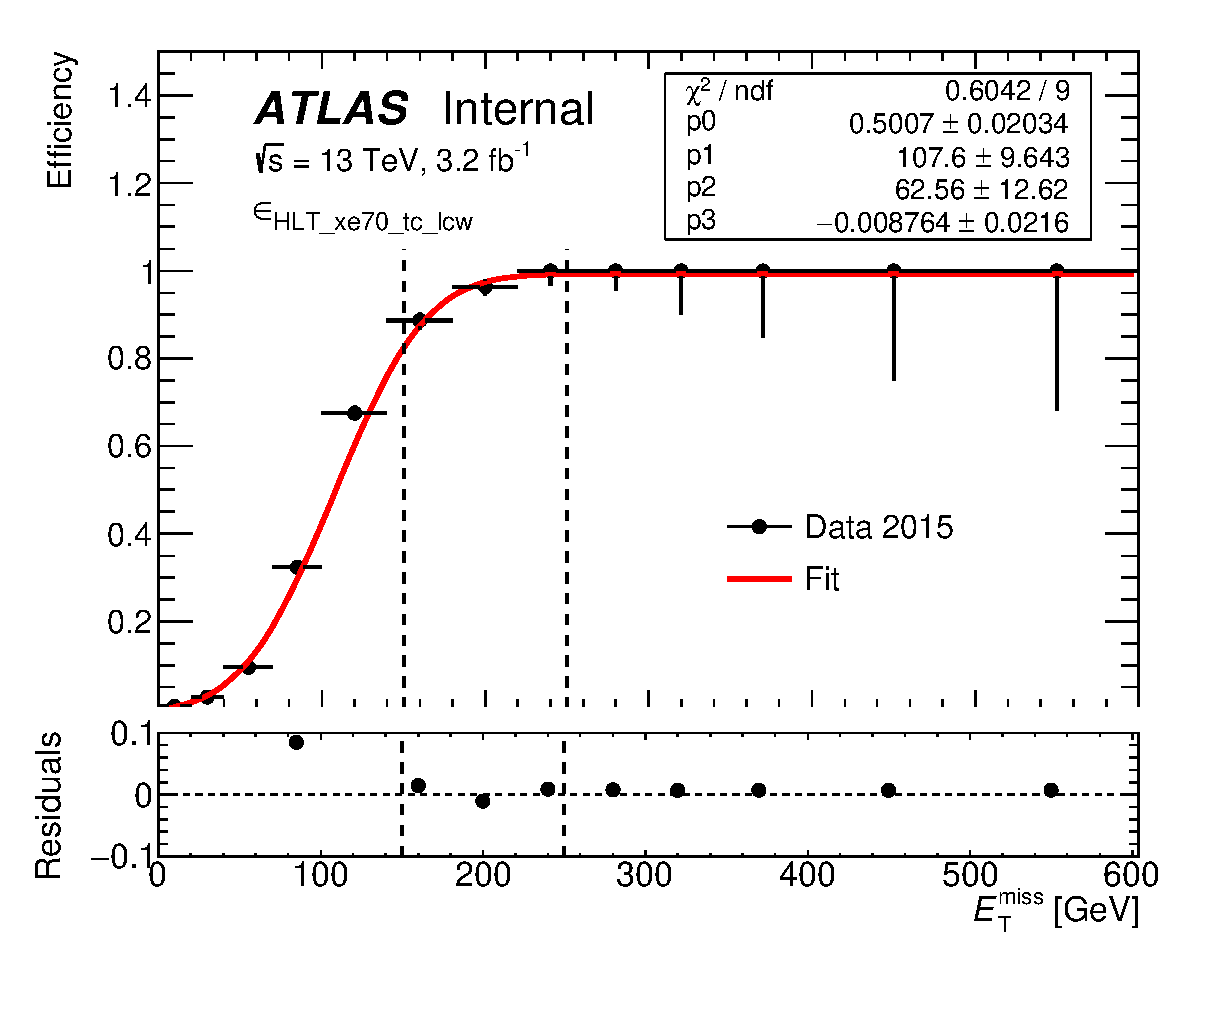
\includegraphics[width=\textwidth]{figures/xe70_tclcw_data15_fitted.eps}
\caption{2015 data-set}
\label{fig:trigFitA}
\end{subfigure} % 
\begin{subfigure}{0.5\textwidth}
   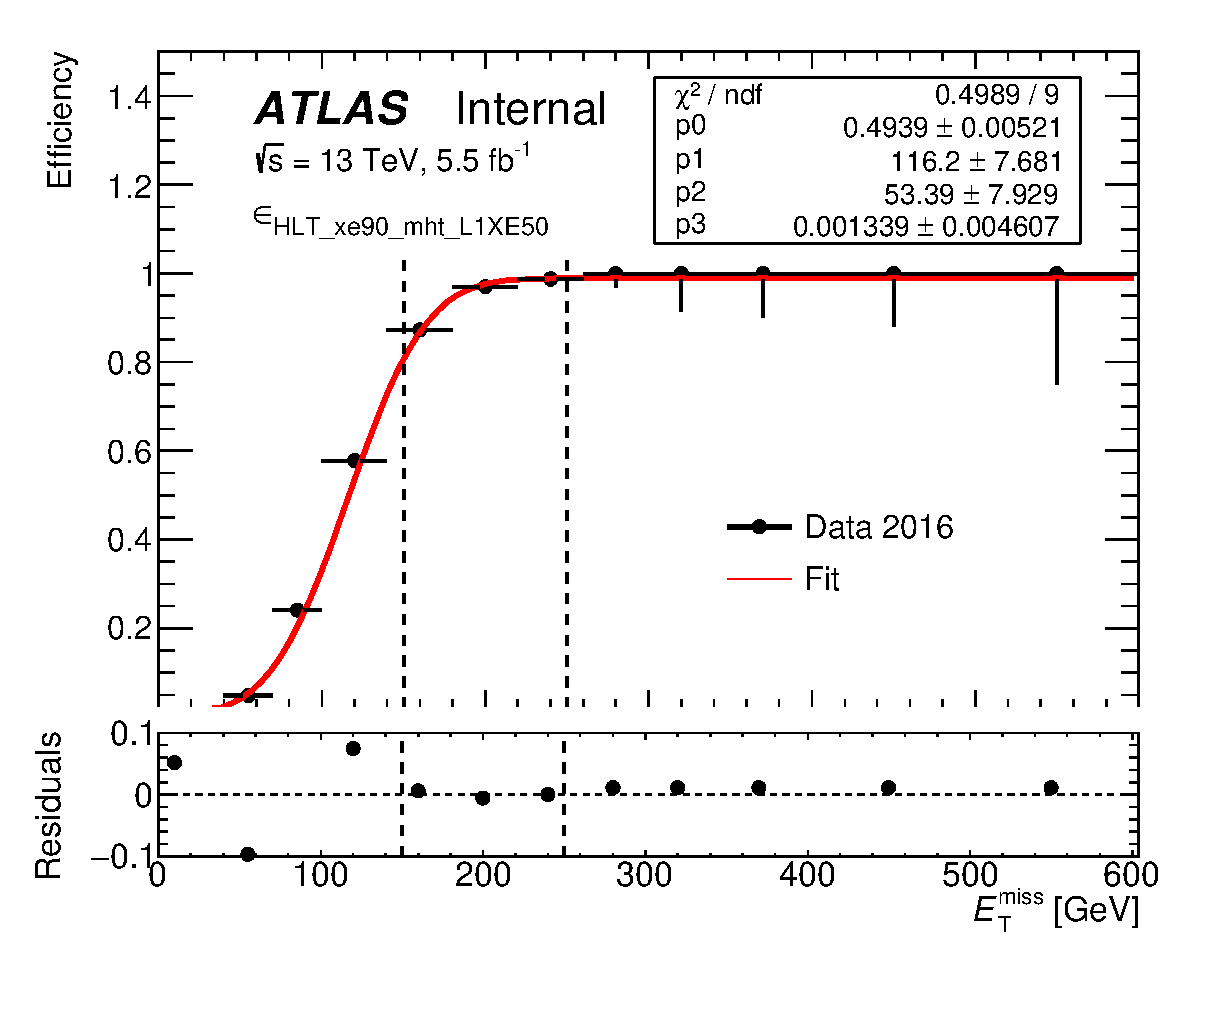
\includegraphics[width=\textwidth]{figures/xe90_mht_data16_fitted.eps}
\caption{2016 data-set}
\label{fig:trigFitB}
\end{subfigure}
\caption{Plots showing trigger efficiency fits}
\end{figure}
